\chapter{The Impact}
\label{ch:15}



\begin{center}
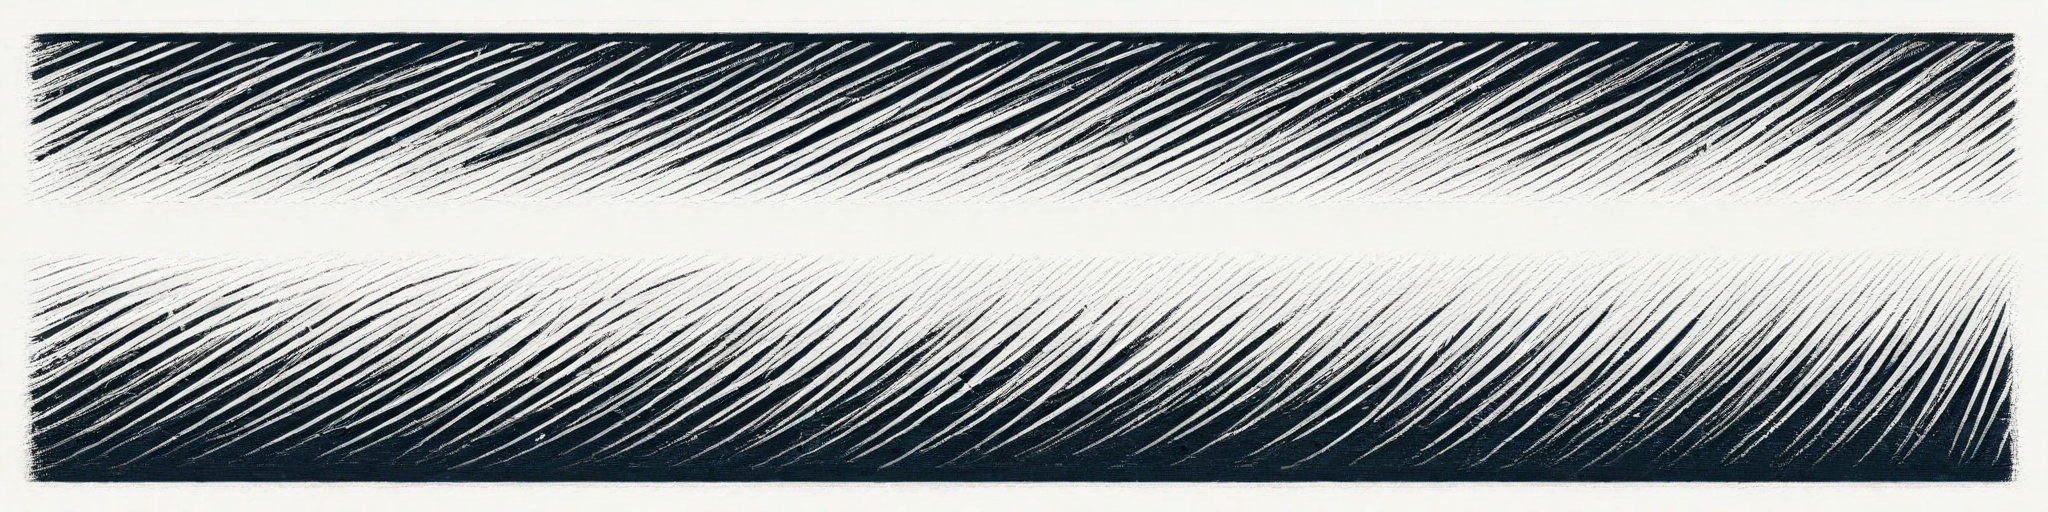
\includegraphics[width=\textwidth]{images/chapterImages/genesis_sketch_00098_.png}
\end{center}

The light came first.

Not from the wrongstar itself but from its interaction with the upper atmosphere. Friction. Compression. Air molecules forced aside at velocities they were never designed to accommodate. The energy of that displacement converting to heat. To light. To radiation across the spectrum.

The sky ignited.

Not gradually. Instantaneously. The entire visible atmosphere became luminous. Brighter than day. Brighter than anything that had existed before. Light that carried heat. Light that was heat. Light that burned.

Aurelia's final thought was observation: the calculations were correct.

The trajectory matched prediction within error margins. The atmospheric interaction was proceeding as modeled. The angle of approach was optimal for maximum global distribution of ejecta. Everything was exactly as the mathematics had determined it would be.

The encoding would survive. The mammals were positioned correctly. The timeline would unfold.

Eight percent.

Sufficient.

The light intensified beyond the capacity of eyes to process. Vision ceased to function. Became irrelevant. The sensory input was just pain signal—too bright, too hot, tissue damage occurring at cellular level.

But consciousness persisted for another moment. Long enough to feel satisfaction. Not happiness. Not peace. Just the mathematical certainty that the equation was balancing exactly as calculated.

The work was complete.

\scenebreak

The sound arrived.

Not heard—felt. A pressure wave moving through air and ground simultaneously. Frequency so low it was more earthquake than noise. The planet itself transmitting the shock of collision. Every molecule between impact point and witness location suddenly displaced, all trying to occupy the space their neighbors had just vacated, creating a cascade of compression that propagated at supersonic velocity.

The gathering scattered like leaves. Bodies lifted and thrown by wind that shouldn't exist. By pressure differential that exceeded any biological resistance. They tumbled through air that was no longer air but plasma. Super-heated. Ionized. Carrying enough energy to flash-cook tissue on contact.

The daughter's consciousness terminated mid-flight. Instant. Clean. No suffering. Just function ceasing as thermal energy exceeded cellular tolerance.

The young female made it three seconds longer. Landed. Tried to run toward her cave half a rotation away. The ground was moving too violently to permit running. She fell. The heat intensified. Her consciousness fragmented—pain signals overwhelming processing capacity. Then nothing. Termination.

The Pair's bodies ignited where they lay. The intertwined necks maintained their position briefly as matter converted to combustion. Then even the physical connection failed. Dispersed. Returned to constituent elements.

Aurelia's body ceased functioning. Organs shut down. Neural activity terminated. The vast cathedral of calculation that had existed behind her eyes—the timelines and probability curves and encoded instructions spanning 65 million years—all of it vanished in an instant.

Consciousness ended.

The universe continued experiencing itself, but not through her.

\scenebreak

The wrongstar struck the planet.

Ten kilometers of nickel-iron traveling at 70,000 kilometers per hour met continental crust three kilometers thick. The physics was straightforward even if the scale was incomprehensible. Kinetic energy converted to heat. Matter compressed beyond tolerance. Bedrock behaving like fluid. Shockwave propagating spherically.

The impact crater formed in seconds. Thirty kilometers deep. Two hundred kilometers across. The ejecta plume rose immediately—millions of tons of vaporized rock and impactor material thrown into ballistic arcs that would carry them halfway around the planet.

The heat pulse ignited everything flammable within a thousand kilometers. Forests became firestorms. Animals became ash. The atmosphere itself burned where oxygen concentration was sufficient.

The shockwave propagated globally. Circles expanding from impact point. When it reached the northern plateau—already empty of witnesses, already cleared of consciousness that could observe it—it scoured the surface clean. The stone patterns scattered. The careful arrangements destroyed. The physical encoding erased.

But the information had already been transferred. Already existed in the genetics of protected populations. Already resided in forty-three locations where small mammals huddled in deep burrows and waited for the shaking to stop.

\scenebreak

In a cave system beneath the western mountains, the tool-using population experienced the impact as darkness and terror and confusion. The ground shook. Rocks fell. Some individuals died crushed. Others injured. The group pressed together in the deepest chambers and waited.

They had no understanding of what was happening. No framework for comprehending planetary-scale catastrophe. Just instinct: hide, wait, survive.

The temperature in the burrow rose but not beyond tolerance. The air grew thin but remained breathable. The shaking eventually stopped. The darkness continued.

They waited.

In their genes, encoded sequences that had been selected for over years waited too. Dormant. Inactive. But present. Ready to express when environmental conditions triggered activation. Ready to unfold across timescales these small creatures couldn't imagine.

Tool use: present and active.
Fire control: dormant, awaiting activation at population density threshold 200,000 years from now.
Agriculture: dormant, awaiting climate stabilization 10,000 years from now.
Language: dormant, awaiting vocal structure evolution.
Mathematics: dormant, awaiting neural development.

On and on. Twenty-seven major thresholds. Hundreds of minor ones. All encoded. All waiting. All positioned in the genome where they would activate on schedule if evolution proceeded along calculated trajectories.

If the population survived. If the traits propagated. If the timeline held.

If.

The tool-users waited in darkness. Some died from injuries sustained in the shaking. Others from stress. The survivors huddled together and waited for the world to make sense again.

It wouldn't make sense for a long time. The impact winter was just beginning. The darkness would persist for months. The cold would intensify. The resources would become scarce. Many would die. Most, probably.

But some would survive. The mathematics said so. The calculations were sound. Eight percent for full success. Ninety-seven percent that something persisted.

The mammals waited. And the code they carried waited with them. Patient. Dormant. Ready.

\scenebreak

The planet convulsed. Volcanism triggered globally by the shockwave's seismic energy. Tsunamis propagating across every ocean. The atmosphere choking with particulate matter. Sunlight blocked. Temperature plummeting. The greenhouse effect reversing to ice house in a matter of weeks.

Ninety-nine point seven percent of large organisms died within the first year. Ninety-four percent of all species extinct within ten years. The world transformed. The climate collapsed. The ecosystems simplified to extremophile survivors and small creatures that could hide and wait and endure.

The dinosaurs vanished completely. Every individual. Every population. Every remnant of the consciousness that had calculated and planned and encoded the future. Gone. Dispersed. Returned to the elements from which they had briefly been organized into pattern.

The mammals endured. Not all of them. Not even most. But enough. In forty-three locations, populations survived the first year. By the second year, thirty-seven populations remained. By the fifth year, twenty-eight. By the tenth year, nineteen.

Nineteen lineages carrying encoded traits. Nineteen populations positioned across the recovering landscape. Nineteen points of potential for the timeline to unfold.

It was enough.

Barely. Just barely. But enough.

\scenebreak

Sixty-five million years later, a woman named Sarah Chen stared at a genetic sequence on a computer screen and felt understanding dawn.

The dinosaurs hadn't just existed. They had planned. Had calculated. Had encoded.

Had loved their world enough to ensure something survived even though they couldn't.

The traits weren't random. The cognitive capabilities weren't evolutionary accidents. Tool use and fire control and agriculture and language and mathematics and astronomy—all programmed. All scheduled. All activated according to a timeline designed before humanity existed.

We were the execution of their code.

The inheritors of a gift we never knew we'd received.

And somewhere in that code, somewhere in the 65-million-year plan that had unfolded exactly as calculated, was an imperative: protect this world. Build the defense grid. Redirect the next asteroid. Ensure consciousness persists.

Ensure something survives.

Pass it forward.

The cycle continues.

\scenebreak

On the northern plateau, long empty of witnesses, wind scattered the last stones. Rain eroded the final configurations. The pattern that had existed dissolved into randomness. The mathematics returned to the landscape from which it had been briefly extracted.

But the understanding persisted. Encoded in living flesh. Written in DNA. Waiting to unfold across geological time.

Aurelia's consciousness had terminated. Her body had dispersed. Her individual existence was complete.

But her work continued. Her calculations propagated forward. Her contribution to collective understanding existed independent of her presence.

The equation had balanced.

Life equaled matter plus pattern plus time.

Consciousness equaled life plus observation plus calculation.

Persistence equaled consciousness plus encoding plus sacrifice.

The variables resolved. The mathematics completed. The timeline began its long, patient unfold toward an uncertain future that was nevertheless calculated with precision.

Eight percent.

Sufficient.

The equation balanced.

\scenebreak

**END OF PART ONE**

